\title{5. Exponenciální a logaritmická funkce}

\author{Jan Peroutka}
\maketitle

\section{Exponenciální a logaritmická funkce}

\subsection{Exponenciální funkce}
Exponenciální funkce je každá funkce tvaru
$$
f(x) = a^x,
$$
kde $a > 0$, $a \ne 1$ a $x \in \mathbb{R}$.

\subsubsection{Vliv základu $a$ na průběh}
\begin{itemize}
    \item Pokud $a > 1$, je funkce rostoucí.
\begin{figure}
            \centering
            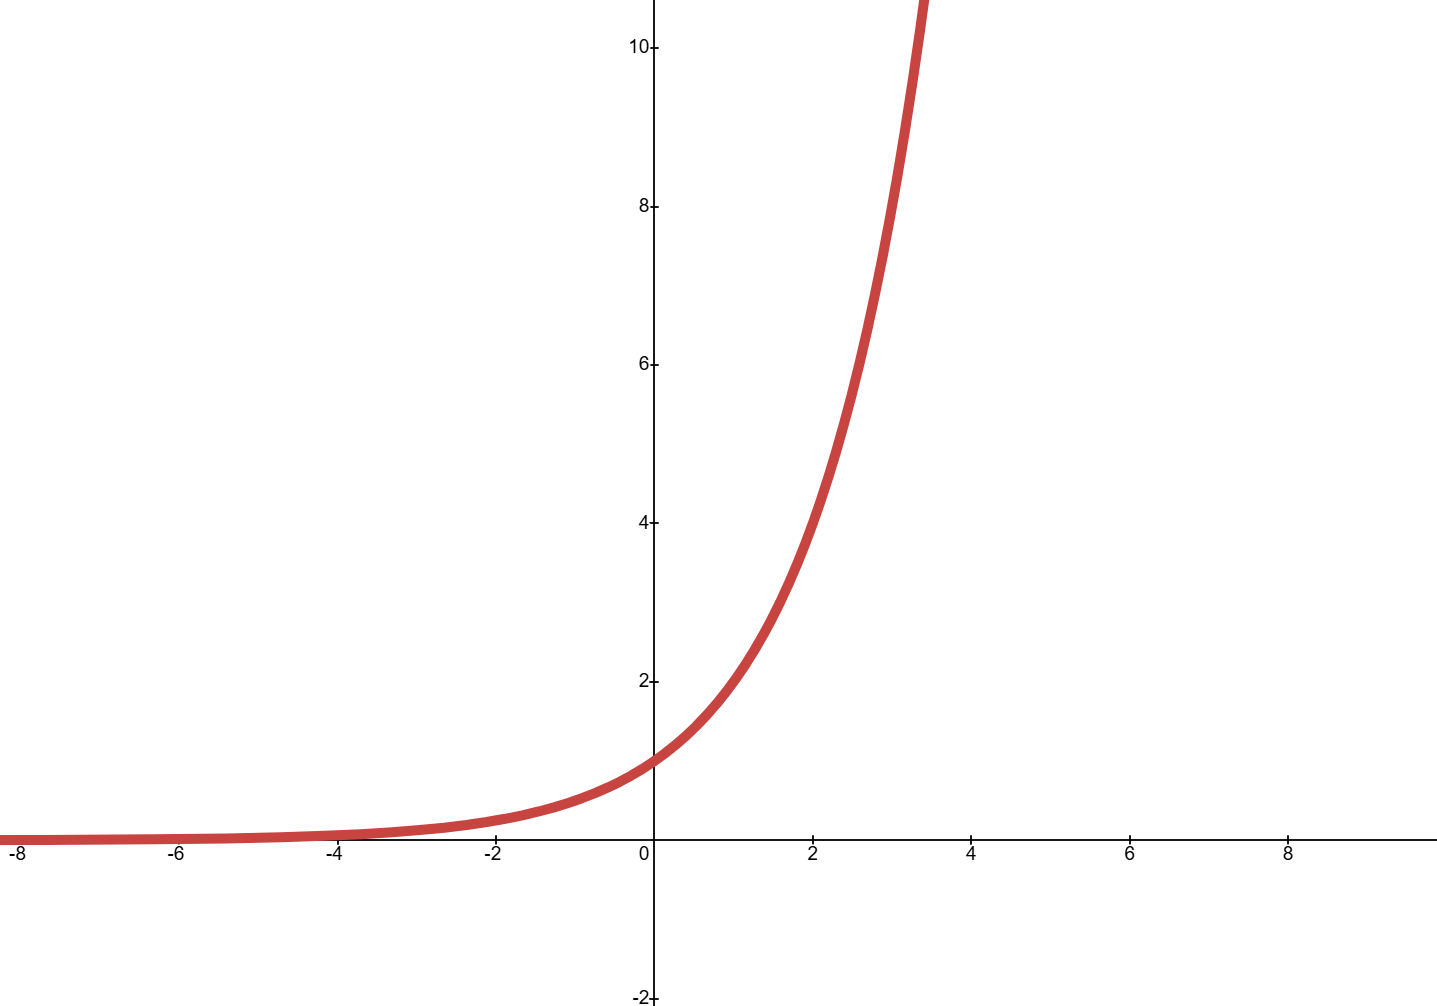
\includegraphics[width=0.5\linewidth]{img/5_exp_ros.png}
            \caption{$y = 2^x$}
        \end{figure}
    \item Pokud $0 < a < 1$, je funkce klesající.
\begin{figure}
    \centering
    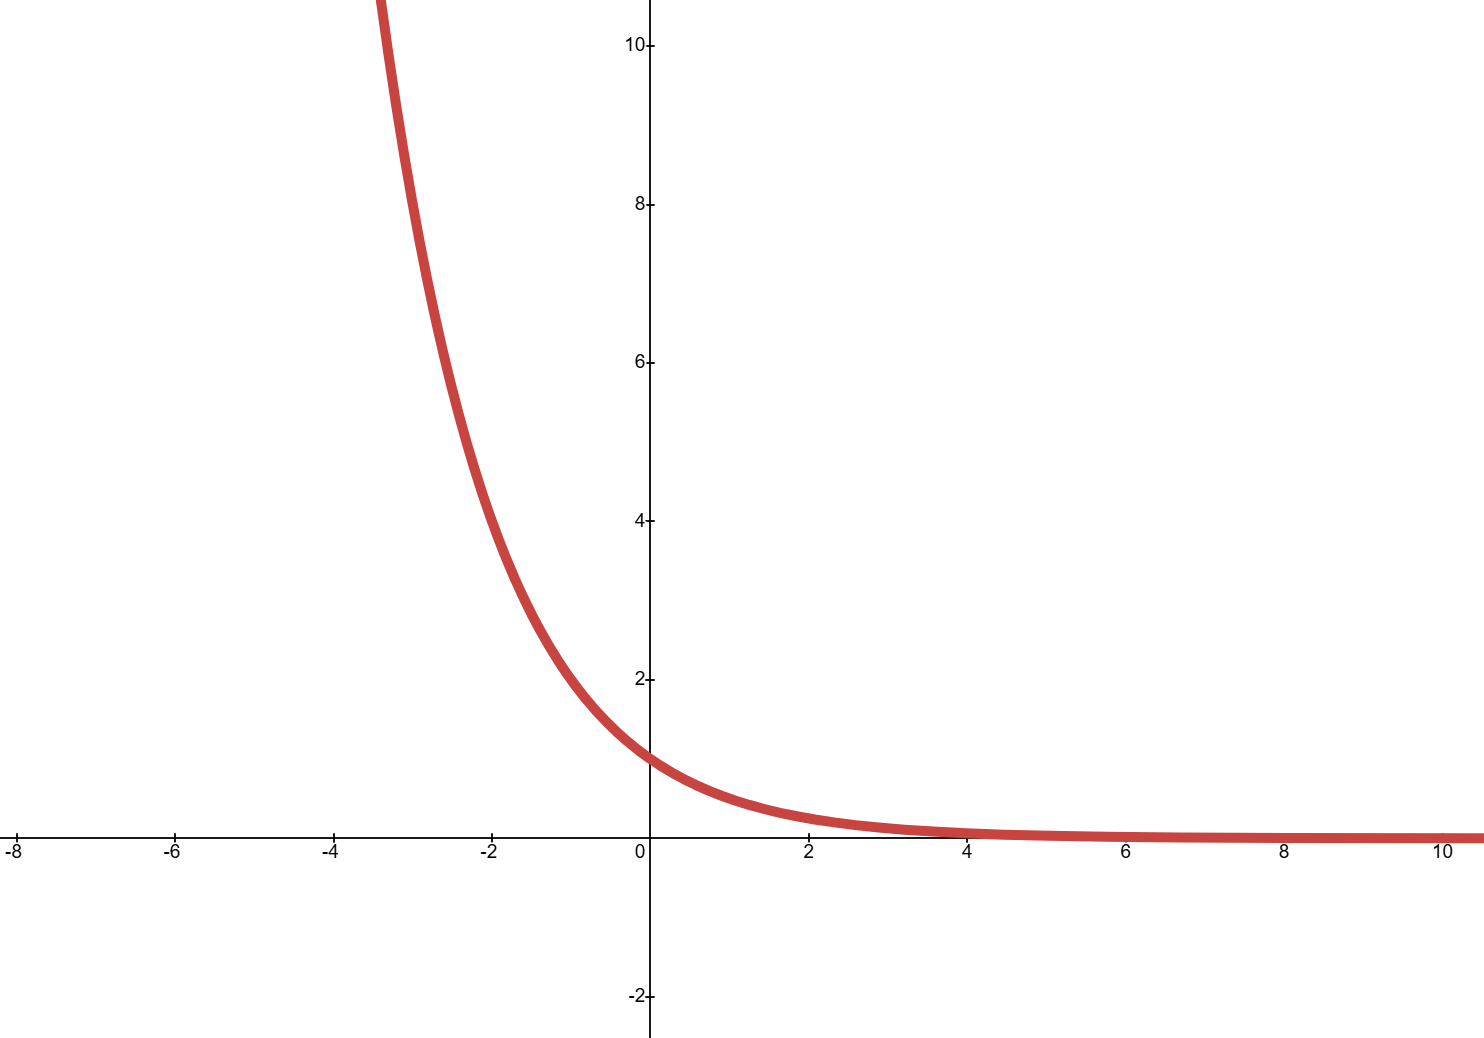
\includegraphics[width=0.5\linewidth]{img/5_exp_kles.png}
    \caption{$y = (\frac{1}{2})^x$}
\end{figure}
\end{itemize}
\textbf{Graf vždy prochází bodem $[0, 1]$.}

\subsubsection{Definiční obor a obor hodnot}
\begin{itemize}
    \item Definiční obor: $D(f) = \mathbb{R}$
    \item Obor hodnot: $H(f) = (0, \infty)$
\end{itemize}

\subsection{Logaritmická funkce}
Logaritmická funkce je inverzní funkcí k exponenciální funkci. Její obecný tvar je:
$$
f(x) = \log_a x,
$$
kde $a > 0$, $a \ne 1$, $x > 0$.

\subsubsection{Vliv základu $a$ na průběh}
\begin{itemize}
    \item Pokud $a > 1$, je funkce rostoucí.
\begin{figure}
        \centering
        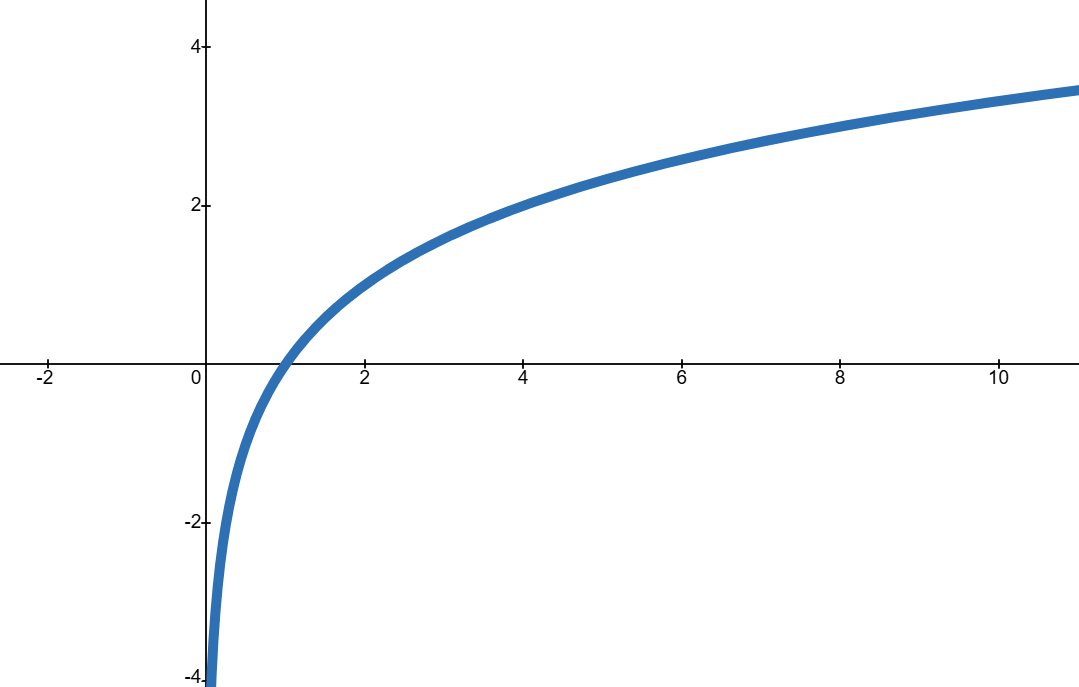
\includegraphics[width=0.5\linewidth]{img/5_log_ros.png}
        \caption{$y=\log_2 x
$}
    \end{figure}
        \item Pokud $0 < a < 1$, je funkce klesající.
\begin{figure}
    \centering
    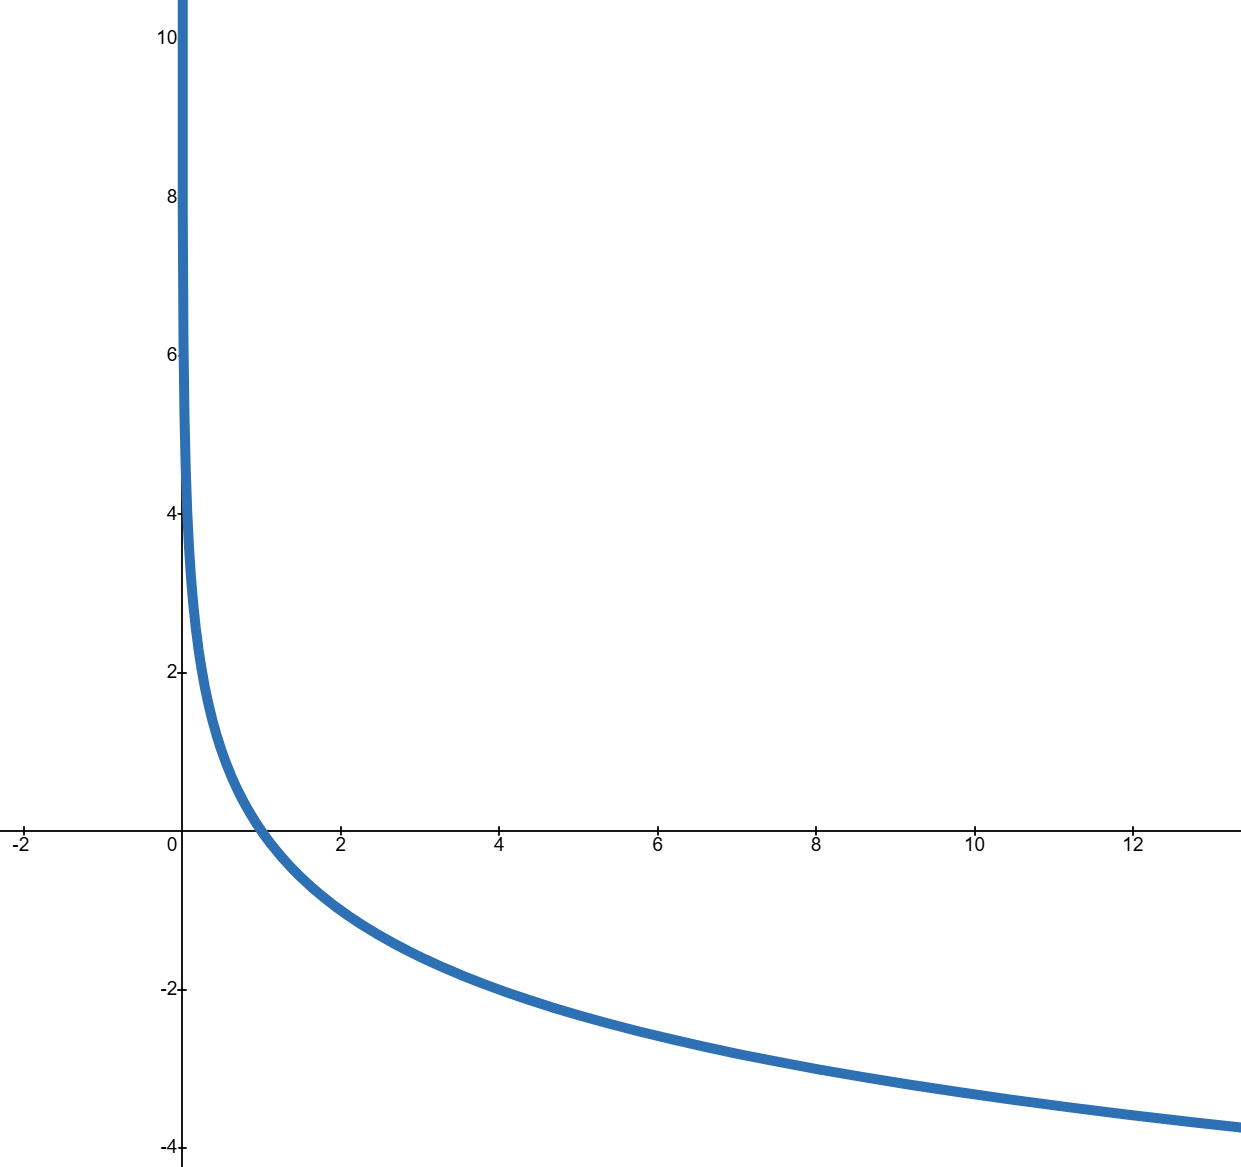
\includegraphics[width=0.5\linewidth]{img/5_log_kles.png}
    \caption{$y=\log_{\frac{1}{2}} x
$}
\end{figure}
\end{itemize}
Graf vždy prochází bodem $[1, 0]$.
\subsubsection{Definiční obor a obor hodnot} 
\begin{itemize}
    \item Definiční obor: $D(f) = (0, \infty)$
    \item Obor hodnot: $H(f) = \mathbb{R}$
\end{itemize} 
\subsection{Vztah mezi exponenciální a logaritmickou funkcí}
Funkce $f(x) = a^x$ a $f^{-1}(x) = \log_a x$ jsou navzájem inverzní. To znamená:
$$
a^{\log_a x} = y \quad \text{a} \quad \log_a(a^x) = y.
$$
Grafy těchto funkcí jsou zrcadlově souměrné podle osy $y = x$.

\subsection{Představa logaritmu}
Logaritmus je odpovědí na otázku: „Na kolikátou musím umocnit číslo $a$, abych dostal číslo $x$?“
$$
\log_a x = y \Leftrightarrow a^y = x.
$$
\subsection{Základní pravidla pro počítání s mocninami a logaritmy}
\subsubsection{Mocniny}
Pro všechna $a > 0$, $m, n \in \mathbb{R}$:
\begin{itemize}
    \item $a^m \cdot a^n = a^{m+n}$
    \item $\frac{a^m}{a^n} = a^{m-n}$
    \item $(a^m)^n = a^{m \cdot n}$
    \item $a^{-n} = \frac{1}{a^n}$
    \item $a^0 = 1$
    \item $\sqrt[n]{a^b} = a^{\frac{b}{n}}$
\end{itemize}

\subsubsection{Logaritmy}
Pro všechna $a, x, y > 0$, $a \ne 1$:
\begin{itemize}
    \item $\log_a(x \cdot y) = \log_a x + \log_a y$
    \item $\log_a\left(\frac{x}{y}\right) = \log_a x - \log_a y$
    \item $\log_a(x^r) = r \cdot \log_a x$
    \item $\log_a a = 1$; $\log_a 1 = 0$
    \item Změna základu: $\log_a x = \frac{\log_b x}{\log_b a}$
\end{itemize}
